\chapter{Frequency Response Analysis of a Single Board Heater System by the Application of Sine Wave}
The aim of this experiment is to do a frequency response analysis of a Single Board Heater System by the 
application of sine wave. The target group is anyone who has basic knowledge of control engineering.


%%%%%%%%%%%%%

\begin{figure}
\centering
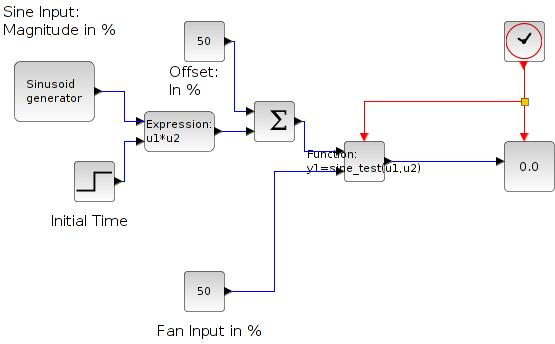
\includegraphics[width=\linewidth]{sinetest_manual/sine_test.jpg}
\caption{Xcos for local Sine Test}
\label{xcos_sine}
\end{figure}

\begin{figure}
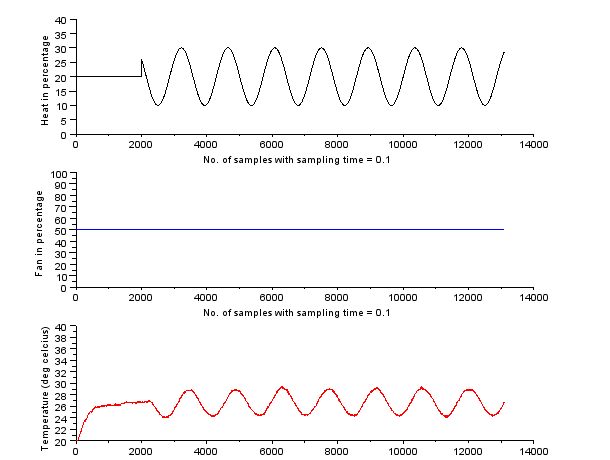
\includegraphics[width=\linewidth]{sinetest_manual/sine-007-plot.png}
\caption{Plot for sine input 0.007Hz}
\label{fig:scope}
\end{figure}

We have used Scilab and Xcos as an interface for sending and receiving data. 
Xcos diagram is shown in figure \ref{xcos_sine}.
The heater current is varied sinusoidally. They are given in percentage of maximum. These inputs can be varied by setting the properties of the input block's properties in Xcos. A provision is made to set the parameters related to it like frequency, amplitude 
and offset. The temperature profile thus obtained is the output. In this experiment we are applying a sine change in the heater current by keeping the fan speed constant. After application of sine change, wait for sufficient amount of time to allow the temperature to reach a steady-state. The plots of their amplitude versus number of collected samples are also available on the scope windows. The output temperature profile, as read by the sensor, is also plotted. The data acquired in the process is stored on the local drive and is available to the user for further calculations.

 In the {\tt sine\_test.xcos} file, open the {\tt sinusoid generator} block's parameters to set the value of sine magnitude and frequency. For the experiment results shown, we have chosen Magnitude = $10$, Frequency = $2*3.14*0.007$. Note that the frequency is to be put in rad/sec. We keep the Phase = $0$. There is also a provision to give the sine input with an offset in amplitude. This can be set using the {\tt Offset} block. We have choosen offset of 20. The time at which the sine input is given after the experiment is started can also be set. This can be done using the {\tt Initial Time} block. Open the {\tt Initial Time} block's parameters. To make the sine input appear after 200 samples of start of the experiment, keep Step time = $200$, Initial Value = $0$ and Final Value = $1$. The initial value and final value will never change for any other value of step time.


\begin{table}
\begin{verbatim}
1.0     20.0       50.0      20.0   1416642805261.0
2.0       20.0       50.0        20.0   1416642806332.0
.
13093.0    28.5       50.0         26.6   1416656557353.0
13094.0     28.5       50.0        26.6   1416656558363.0
\end{verbatim}
\caption{Data obtained after application of sine input of $0.007Hz$}
\label{sinedata}
\end{table}

The sine test data file will be saved in {\tt Sine\_Test} folder. The name of the file will be the date and time at which the experiment was conducted. A sample data file is provided in the same folder. The sample data file is named as {\tt sine-data-local.txt} and {\tt sine-data-virtual.txt}. Refer to the one depending on wheather you are performing a local or a virtual experiment. Referring to the data file thus obtained as shown in table \ref{sinedata}, the first column in this table denotes samples. The second column in this table denotes heater in percentage. It starts at 20 and then varies sinosoidally. The third column denotes the fan in percentage. It has been held constant at 50 percent. The fourth column refers to the value of temperature. The fifth column denotes time stamp. The virtual data file will have four time stamp columns apart from first 3 columns. These four time stamp columns are client departure, server arrival, server departure and client arrival. These can be used for advanced control algorithms. These additional time stamps exist in virtual mode because of the presense of network delay.

\section{Conducting Sine Test on SBHS locally}
The detailed procedure to perform a local experiment is explained in Chapter\ref{sercomm}. A summary of the same is provided in section \ref{local-summary} It is same for this section with following changes.

\begin{enumerate}
\item Step1: The working directory is {\tt  Sine\_test}
\item Step2: Same
\item Step3: Same
\item Step4: Same
\item Step5: Load sine test function by executing command\\ {\tt exec<space>sine\_test.sci}
\item Step6: Load Xcos code for sine test using the command\\ {\tt exec<space>sine\_test.xcos}
\item Step7: Same
\end{enumerate}


\section{Conducting Sine Test on SBHS, virtually}
The detailed procedure to perform a local experiment is explained in Chapter\ref{virtual}. A summary of the same is provided in section \ref{vlabsexpt}. It is same for this section with following changes.

\begin{enumerate}
\item Step1: The working directory is {\tt  SineTest}. Open this directory.
\item Step2: Same
\item Step3: Same
\item Step4:  Switch to the SineTest experiment directory and double-click on the file {\tt sinetest.sce}. This will launch scilab and also open the file {\tt sinetest.sce} in the scilab editor. Linux users will have to launch scilab manually. They also have to change the working directory to {\tt  SineTest} and then open the {\tt  sinetest.sce} file in the scilab editor.
\item Step5: Same
\item Step6: Execute the file {\tt sinetest.sce}.  Expect the sine test xcos diagram to open automatically. If this doesnt happen, check the scilab console for error message.
\item Step7: Execute the sinetest xcos diagram.
\item Step8: Same
\end{enumerate}


 The virtual experiment response is shown in figure \ref{sine-virtual}. The corresponding data file is shown in table \ref{sinedata}. The time stamps shown are cut short for better viewing. This data file can be found in {\tt SineTest} folder for virtual experiments. The name of this file is {\tt sine-data-virtual.txt}.


\begin{figure}
\centering
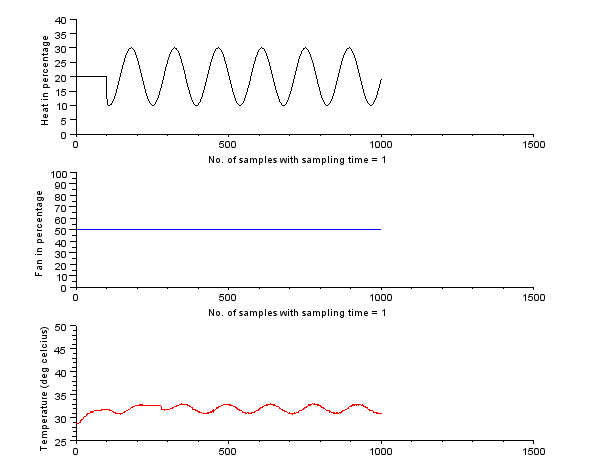
\includegraphics[width=\linewidth]{sinetest_manual/sine-plot-virtual-007.png}
\caption{Sine test Virtual experiment response}
\label{sine-virtual}
\end{figure}


\begin{table}
\begin{verbatim}
0 0 100 28.80 14...4739 14...6427 14...6445 14...4786 0.10000E+01
1 20 50 28.90 14...5247 14...6938 14...6956 14...5294 0.10000E+01
.
.
999 18 50 31.00 14...2253 14...3973 14...3990 14...2299 0.99900E+03
1000 19 50 31.00 14...3268 14...4989 14...5007 14...3315 0.10000E+04
\end{verbatim}
\caption{Sine data obtained after performing virtual Sine Test}
\label{rampdata}
\end{table}

%%%


\section{Frequency Analysis of sine test data}
 Frequency response of a system means its steady-state response to a sinusoidal input. 
 For obtaining a frequency response of a system, we vary the frequency of the input signal over a spectrum of interest. 
 The analysis is useful and simple because it can be carried out with the available signal generators and measuring devices. Let us see the theory and procedure.  Please note that this procedure is common for data obtained using both local and virtual experiments.

Consider a sinusoidal input
\begin{align}
U(t) &= Asin \omega t
\intertext{The Laplace transform of the above equation yields}
U(s) &= \frac{A\omega}{s^2 + \omega^2} \label{lap_tran}
\intertext{Consider the standard first order transfer function given below}
G(s) &= \frac {Y(s)}{U(s)} = \frac K{s + 1}
\intertext{Replacing the value of U(s) from equation \ref{lap_tran}, we get}
Y(s) &= \frac{KA\omega}{(\tau s + 1)(s^2 + \omega ^2)}\\
&=\frac{KA}{\omega ^2\tau ^2 + 1}\left[\frac{\omega \tau ^2}{\tau s +1}- \frac{\tau s \omega}{s^2 + \omega^2}+\frac{\omega}
{s^2 + \omega^2}\right]
\intertext{Taking Laplace Inverse, we get}
y(t) &= \left[\frac {KA}{\omega^2\tau^2+ 1}\right]\left[\omega \tau e^{\frac {-t}{\tau}}-\omega \tau cos(\omega t)+
sin(\omega t)\right] 
\intertext{The above equation has an exponential term $e^\frac{-t}{\tau}$. Hence, for large value of time, its value will 
approach to zero and the equation will yield a pure sine wave. One can also use trigonometric identities to make the equation 
look more simple.}
y(t) &= \left[\frac{KA}{\sqrt{\omega^2 \tau^2 + 1}}\right]\left[sin (\omega t) + \phi \right]
\intertext{where,}
\phi &= -tan^{-1}(\omega \tau)
\intertext{By observing the above equation, one can easily make out that for a sinusoidal input the output is also sinusoidal
but has some phase difference. 
Also, the amplitude of the output signal, $\hat{A}$, has become a function of the input signal frequency, $\omega$.}
\hat{A}&=\frac{KA}{\sqrt{\omega^2 \tau^2 + 1}}
\intertext{The amplitude ratio (AR) can be calculated by dividing both sides by the input signal amplitude A.}
AR &=\frac{\hat{A}}{A}=\frac{K}{\sqrt{\omega^2 \tau^2 + 1}}
\intertext{Dividing the above equation by the process gain K yields the normalized amplitude ratio $(AR_n)$}
AR_n &=\frac{AR}{K}=\frac{1}{\sqrt{\omega^2 \tau^2 + 1}}
\end{align}
Because the process steady state gain is constant, the normalized amplitude ratio is often used for 
frequency response analysis \cite{dale04}.

\subsection{Procedure}
Now let us calculate amplitude ratio and phase difference. 

\begin{enumerate}
\item Download the Analysis folder from the sbhs website. It will be available under {\tt downloads} section.  Download the file for {\tt SBHS Analysis Code (local \& virtual)}. The name of the file is {\tt scilab\_codes\_analysis}. The download will be in zip format. Extrat the downloaded zip file. You will get a folder {\tt scilab\_codes\_analysis}. 
\item Open the {\tt scilab\_codes\_analysis} folder and then locate and open the folder {\tt Sine\_Analysis}.
 \item Copy the sine test data file to this folder.
 \item Change the Scilab working directory to  {\tt Sine\_Analysis}
 \item Open the file {\ttfamily sine-analysis.sce} in scilab editor and enter the name of the data file (with extention) in the {\tt filename} field.
\item Put the value of frequency {\ttfamily f} for the calculation of amplitude ratio and phase difference and execute it. Here {\ttfamily f} means input frequency.
\item Expect the values of amplitude ratio and phase difference on the scilab console.
\end{enumerate}

  
\begin{figure}
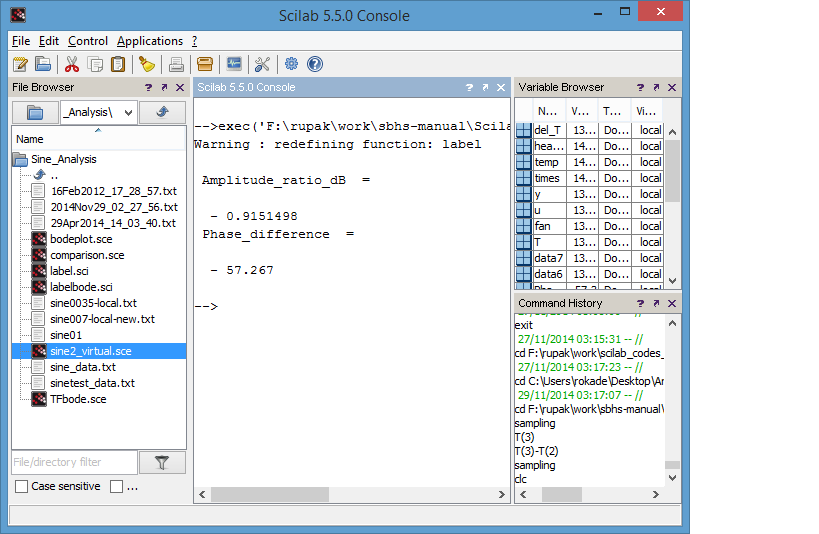
\includegraphics[width=\linewidth]{sinetest_manual/sine-local-analysis-console.png}
\caption{Amplitude ratio and Phase difference for local data file}
\label{scilab_op}
\end{figure}
The results shown are for the data file {sine-data-local.txt}. It could be seen from figure \ref{scilab_op} that the amplitude ratio turns out to be $-0.915$dB and phase difference to be $-57.267$\textdegree.
The plot thus obtained is shown in figure \ref{plot0.4}
\begin{figure}
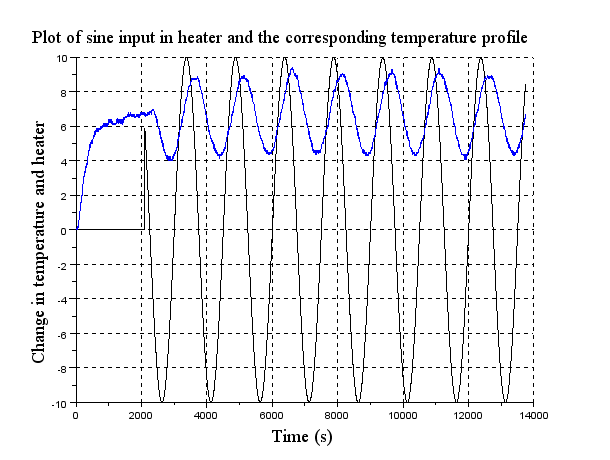
\includegraphics[width=\linewidth]{sinetest_manual/sine-local-analysis}
\caption{Plot of Input and Output vs time}
\label{plot0.4}
\end{figure}

Repeat this calculation over a range of frequencies and note down the values of amplitude ratio in dB and phase difference. 
Input these values for the appropriate frequencies into the Scilab code {\ttfamily TFbode.sce} and execute it to get a 
Bode plot of the plant which is illustrated in figure \ref{bode_plot}.
\begin{figure}
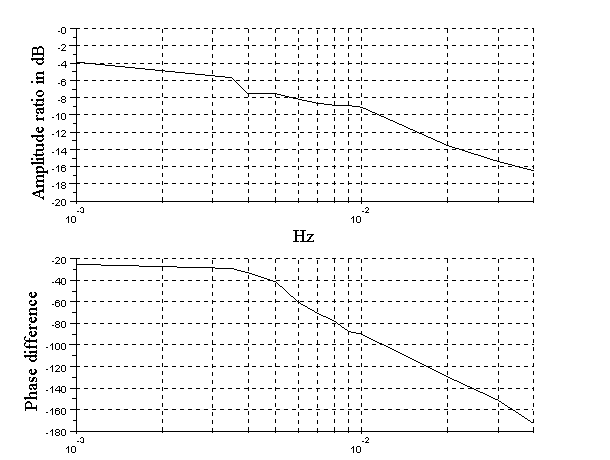
\includegraphics[width=\linewidth]{sinetest_manual/bodeplot}
\caption{Bode plot obtained from the plant}
\label{bode_plot}
\end{figure}

Bode plot can be obtained directly from the plant's second order transfer function \cite{kmm09} with the help of Scilab code
{\ttfamily TFbode.sce}, as shown in figure \ref{tfbode}. A visual comparison of the two Bode plots can be done to 
validate the Bode diagram obtained from the plant.
\begin{figure}
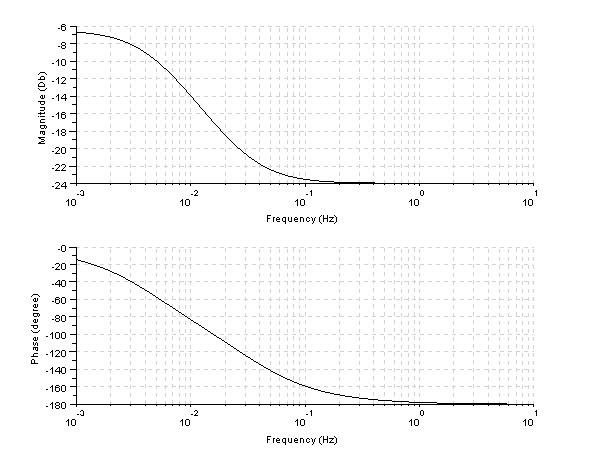
\includegraphics[width=\linewidth]{sinetest_manual/plant_bode_tf}
\caption{Bode plot obtained through plant's transfer function}
\label{tfbode}
\end{figure}

To compare the two plots, we plot it on the same graph as shown in figure \ref{compare_bode}
\begin{figure}
\centering
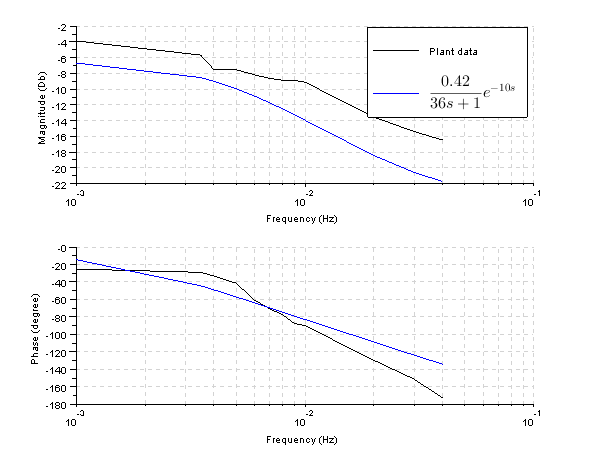
\includegraphics[width=\linewidth]{sinetest_manual/bode_comparison}
\caption{Comparison of Bode plots}
\label{compare_bode}
\end{figure}



\section{Scilab Code}\label{sinecodes}

\begin{code}
\ccaption{sine\_test.sci}{\ttfamily sine\_test.sci}
\lstinputlisting{Scilab/local/Sine_Test/sine_test.sci}
\end{code}


\begin{code}
\ccaption{sinetest.sce}{\ttfamily sinetest.sce}
\lstinputlisting{Scilab/virtual/SineTest/sinetest.sce}
\end{code}

\begin{code}
\ccaption{sinetest.sci}{\ttfamily sinetest.sci}
\lstinputlisting{Scilab/virtual/SineTest/sinetest.sci}
\end{code}

\begin{code}
\ccaption{sine2.sce}{\ttfamily sine-analysis.sce}
\lstinputlisting{Scilab/Analysis/Sine_Analysis/sine-analysis.sce}
\end{code}

\begin{code}
\ccaption{lable.sci}{\ttfamily label.sci}
\lstinputlisting{Scilab/Analysis/Sine_Analysis/label.sci}
\end{code}

\begin{code}
\ccaption{bodeplot.sce}{\ttfamily bodeplot.sce}
\lstinputlisting{Scilab/Analysis/Sine_Analysis/bodeplot.sce}
\end{code}


\begin{code}
\ccaption{labelbode.sci}{\ttfamily labelbode.sci}
\lstinputlisting{Scilab/Analysis/Sine_Analysis/labelbode.sci}
\end{code}


\begin{code}
\ccaption{TFbode.sce}{\ttfamily TFbode.sce}
\lstinputlisting{Scilab/Analysis/Sine_Analysis/TFbode.sce}
\end{code}

\begin{code}
\ccaption{comparison.sce}{\ttfamily comparison.sce}
\lstinputlisting{Scilab/Analysis/Sine_Analysis/comparison.sce}
\end{code}

%\begin{code}
%\ccaption{sine2\_virtual.sce}{\ttfamily sine2\_virtual.sce}
%\lstinputlisting{Scilab/Analysis/Sine_Analysis/sine2_virtual.sce}
%\end{code}

